% !TEX root = ./2nde.tex
\begin{exo}
	Le kendo est un art martial traditionnel japonais qui se pratique principalement avec un shinai, un sabre de bambou.

	Ci-dessous, on a tracé le diagramme en boîte portant sur la masse (en g) d'un échantillon de shinais fabriqués par Kumamoto.
	\vspace*{2mm}
	\begin{center}
		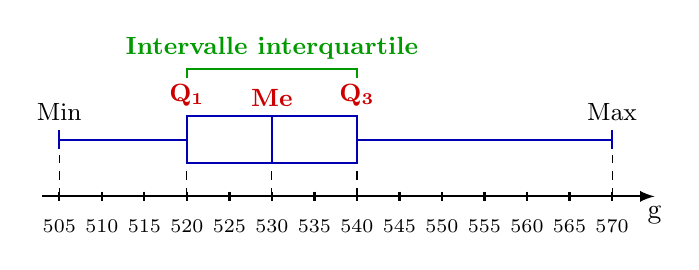
\begin{tikzpicture}[scale=0.6, x=0.18cm, y=1cm, >=latex]
			% Axe des graduations
			\draw[->, thick] (503,0) -- (575,0) node[below] {g};

			% Graduations de 5 en 5 et les labels
			\foreach \x in {505, 510, 515, 520, 525, 530, 535, 540, 545, 550, 555, 560, 565, 570} {
					\draw[thick] (\x, 0.1) -- (\x, -0.1) node[below=3pt] {\scriptsize \x};
				}

			% Lignes pointillées verticales de rappel vers l'axe
			\draw[dashed] (505,0) -- (505,1);
			\draw[dashed] (520,0) -- (520,0.7);
			\draw[dashed] (530,0) -- (530,0.7);
			\draw[dashed] (540,0) -- (540,0.7);
			\draw[dashed] (570,0) -- (570,1);

			% Boîte interquartile (Q1 à Q3)
			\draw[thick, blue!70!black] (520,0.7) rectangle (540,1.7);
			% Médiane (Me)
			\draw[thick, blue!70!black] (530,0.7) -- (530,1.7);

			% Moustaches (Min à Q1 et Q3 à Max)
			\draw[thick, blue!70!black] (505,1.2) -- (520,1.2);
			\draw[thick, blue!70!black] (540,1.2) -- (570,1.2);

			% Bornes des moustaches (traits verticaux Min et Max)
			\draw[thick, blue!70!black] (505,1.0) -- (505,1.4);
			\draw[thick, blue!70!black] (570,1.0) -- (570,1.4);

			% Textes explicatifs au-dessus du diagramme
			\node[above, font=\small] at (505,1.4) {Min};
			\node[above, font=\small\bfseries, red!80!black] at (520,1.7) {Q\textsubscript{1}};
			\node[above, font=\small\bfseries, red!80!black] at (530,1.7) {Me};
			\node[above, font=\small\bfseries, red!80!black] at (540,1.7) {Q\textsubscript{3}};
			\node[above, font=\small] at (570,1.4) {Max};

			% Crochet d'intervalle interquartile
			\draw[thick, green!60!black] (520,2.5) -- (520,2.7) -- (540,2.7) -- (540,2.5);
			\node[above, font=\small\bfseries, green!60!black] at (530,2.7) {Intervalle interquartile};
		\end{tikzpicture}
	\end{center}

	\begin{enumerate}
		\item Lire la valeur de la médiane puis en donner une interprétation.
		\item Écrire trois phrases commençant par : \begin{center}\og{} Environ 50 \% des shinais ont une masse comprise entre \dots \fg{}\end{center}
		\item Calculer l'écart interquartile.
		\item Pour être homologué, la masse d'un shinai doit dépasser 510 g. Que penser de la production de Kumamoto ?
	\end{enumerate}
\end{exo}
